\documentclass[11pt]{article}

\usepackage[margin=0.9in]{geometry}
\usepackage{amsmath,amssymb,amsthm,mathtools}
\usepackage{booktabs,array,longtable}
\usepackage{graphicx}
\usepackage{caption}
\usepackage{subcaption}
\usepackage{placeins}
\usepackage{hyperref}
\usepackage{enumitem}
\usepackage{xcolor}
\usepackage[authoryear,round]{natbib}

\hypersetup{colorlinks=true, linkcolor=blue, urlcolor=blue, citecolor=blue}
\allowdisplaybreaks

\newtheorem{theorem}{Theorem}
\newtheorem{proposition}{Proposition}
\newtheorem{corollary}{Corollary}
\newtheorem{lemma}{Lemma}
\newtheorem{remark}{Remark}
\newcommand{\R}{\mathbb{R}}
\newcommand{\N}{\mathcal{N}}
\newcommand{\one}{\mathbf{1}}
\newcommand{\op}{\mathrm{op}}
\newcommand{\argmax}{\operatorname*{arg\,max}}
\newcommand{\argmin}{\operatorname*{arg\,min}}

\title{Capital-Level Factor Neutrality with Projected Partial Rebalancing}
\author{Anonymous Author(s)}
\date{}

\begin{document}
\maketitle

\begin{abstract}
Active managers often remove factor exposure from alpha signals before portfolio construction.  This
signal-level operation is useful for interpretation, but it does not generally imply that the implemented
portfolio is factor-neutral after risk scaling, clipping, gross normalisation, volatility targeting, or partial
rebalancing.  This paper studies a portfolio-construction method that imposes neutrality directly on the
capital weights that are actually traded.

At each rebalance, an exposure matrix $F_t$ defines the monitored neutral subspace
$\ker F_t^\top$.  The portfolio is written as $u_t=Q_t\theta_t$, where the columns of $Q_t$ form an
orthonormal basis of this subspace.  Optimisation is therefore carried out in neutral coordinates, so every
feasible portfolio satisfies the factor-neutrality equations on the implemented capital vector.  The same
representation gives a direct equality-constrained Markowitz interpretation and finite-sample exposure
leakage bounds when the construction and monitoring exposure matrices differ.

The paper also introduces a projected partial-rebalancing rule.  Before trading toward the new neutral
target, the previous holding is projected into the current neutral subspace; the portfolio is then moved
part way toward the full neutral target.  Since both endpoints are neutral under the current exposure
matrix, the entire interpolation path remains neutral.

Walk-forward tests across six research universes compare ordinary alpha, residualised alpha, the full
neutral target, and projected partial neutral-coordinate portfolios.  The results are used as construction
diagnostics: neutral-coordinate portfolios exhibit numerical-level exposure leakage, while projected
partial variants reduce turnover relative to the full neutral target.  The empirical section evaluates
exposure control, turnover, and implementation stability under fixed validation choices.
\end{abstract}

\noindent\textbf{Keywords:} portfolio construction; factor neutrality; turnover control;
constrained Markowitz optimisation; transaction costs; walk-forward validation.

\section{Introduction}

Active portfolio management separates forecasting from construction.  A forecasting model produces
scores, expected-return proxies, or rankings; the construction process converts those inputs into capital
weights subject to risk, leverage, turnover, benchmark, liquidity, and factor-exposure controls.  A common
practice is to residualise the alpha signal against style, sector, beta, volatility, or other characteristics
before optimisation.  That operation can clarify the signal, but it does not control the exposures of the
implemented capital vector.  Risk weighting, clipping, gross normalisation, volatility targeting, and
partial rebalancing can all reintroduce factor exposure.

For an active sleeve, overlay, or monitored mandate, the relevant question is whether the traded capital
vector satisfies the exposure equations after all construction steps have been applied.  The problem is
finite-sample and dynamic: the investable universe, exposure matrix, risk estimate, and neutral subspace
change through time.

At rebalance time $t$, let $F_t\in\R^{n_t\times m_t}$ be the chosen exposure matrix.  Its columns may
contain sector indicators, style scores, beta estimates, volatility characteristics, nonlinear transformations
of characteristics, or any other exposure directions to be removed.  A capital vector $u_t\in\R^{n_t}$ is
neutral when
\[
        F_t^\top u_t=0.
\]
In words, the dollar-weighted exposure of the implemented active portfolio to each selected exposure
column is zero.
Rather than residualising the signal and then optimising in the original asset coordinates, we compute an
orthonormal basis $Q_t$ of $\ker F_t^\top$ and optimise over
\[
        u_t=Q_t\theta_t.
\]
Thus the optimisation variables $\theta_t$ are coordinates inside the neutral capital space; any feasible
coordinate vector automatically produces a neutral capital vector.
This neutral-coordinate representation distinguishes capital-space neutrality from signal-space
residualisation: the feasible capital vectors are neutral, not just the forecasting input.

Turnover is the second issue.  A fully reoptimised neutral target can move sharply when signals,
covariances, or exposure definitions change.  Projected partial neutral-coordinate rebalancing first projects the old
holding into the current neutral subspace and then chooses a point on the line segment to the full
neutral target.  A one-dimensional utility calculation selects the interpolation coefficient.  Since both
endpoints lie in the current neutral subspace, the interpolation remains neutral.

The contribution is a finite-sample construction protocol rather than an alpha model or covariance
estimator.  The null-space representation itself is a standard linear-algebraic device.  Its role here is to
make neutrality a property of the implemented capital vector after optimisation, normalisation, overlays,
and partial-trading rules have entered the process.  This distinction matters in practice because
residualised signals can still lead to non-neutral portfolios once these steps are applied.

The paper makes three specific points.  First, capital-level neutrality should be imposed and monitored
on the final portfolio weights, not inferred from a residualised forecasting signal.  Second, neutral
coordinates give a simple finite-sample implementation of equality-constrained portfolio construction
and make ex-post exposure checks transparent.  Third, when the exposure matrix changes through time,
partial rebalancing should begin by projecting the previous holding into the current neutral subspace;
otherwise a turnover-saving rule can carry stale exposure into the new period.

The empirical analysis tests these construction claims using walk-forward research panels.  The tests ask
whether the proposed construction enforces the monitored exposure constraints after optimisation and
rebalancing, and whether partial rebalancing can reduce turnover while preserving capital-level
neutrality.  The fixed validation specification uses a cubic volatility-exposure matrix, while the theory
applies to any user-chosen finite exposure matrix.  The empirical role of the tests is to validate the
construction layer rather than to rank alpha models.

\section{Related literature and positioning}

The paper is related to mean--variance portfolio construction, constrained optimisation, and active factor
control.  The starting point is \citet{Markowitz1952}.  Subsequent work shows that estimation error,
constraints, and implementation rules can materially affect realised portfolios; see, for example,
\citet{Michaud1989}, \citet{DeMiguel2009}, and \citet{Kolm2014}.  Covariance shrinkage and portfolio
constraints are often used to stabilise realised allocations
\citep{LedoitWolf2004,JagannathanMa2003}.  Transaction costs and rebalancing rules are also central in
practical portfolio construction \citep{Lobo2007,Boyd2017}.

The paper is also related to active portfolio management and factor-neutral mandates.  In practice,
alpha signals may be residualised against sector, style, beta, volatility, liquidity, or other exposure
variables before optimisation; see \citet{GrinoldKahn2000} and \citet{ClarkeDeSilvaThorley2002}.  Such
residualisation is useful for signal interpretation and for diagnosing whether a forecast is mainly a proxy
for known characteristics.  It is not, however, the same as constraining the traded capital vector.  A risk
model, leverage rule, gross normalisation, volatility overlay, clipping rule, or partial-rebalancing rule can
change the exposures of the implemented book.

The method is a portfolio-construction module.  It does not replace the forecasting model, covariance
estimator, transaction-cost model, or risk system.  Given an exposure matrix, it enforces neutrality on
the portfolio weights produced by the construction process.  The point is not the existence of
equality-constrained optimisers, but where the constraint is imposed and how stale exposure is handled
under partial rebalancing.

\section{Asset-management workflow and use case}

The method is intended as a factor-neutral construction module. The manager first chooses the exposure
matrix $F_t$ to be neutralised. Its columns may include sector indicators, style scores, beta estimates,
volatility characteristics, liquidity variables, or nonlinear transformations of such variables. The neutral
basis $Q_t$ is then computed using information available before the holding period.

For an asset manager, the relevant audit object is the implemented portfolio, not the raw forecast.  A
signal may be orthogonal to the monitored exposures at the forecasting stage and still produce a book
with nonzero exposure after risk weighting, gross normalisation, volatility targeting, or partial trading.
The proposed workflow treats factor neutrality as a post-construction requirement: the exposure check is
applied to the capital vector that would actually be traded.

The intended use case is an active sleeve or overlay in which neutrality is monitored after optimisation
and rebalancing.  The alpha vector and risk estimate are projected into the neutral capital space to obtain
a full neutral target.  The previous holding is separately projected into the current neutral subspace, and
the final portfolio moves part way from the projected old holding to the new full target.  The monitor
records exposure leakage, turnover, the selected rebalancing coefficient, ex-ante risk, conditioning,
drawdown, numerical rank, and implementation flags at each rebalance.

This separates three implementation choices: the forecasting signal, the exposure policy, and the speed
of rebalancing.  In an existing portfolio-construction system, the method can be inserted after signal
generation and before trade generation: choose the monitored exposure matrix, compute the neutral
target, project the old holding into the current neutral subspace, select the rebalancing coefficient, and
monitor realised exposure leakage and turnover.  The guarantees apply to the exposure columns included
in $F_t$.

\begin{center}
\fbox{
\begin{minipage}{0.92\linewidth}
\textbf{Projected partial neutral-coordinate rebalancing.}

At rebalance time $t$:
\begin{enumerate}[leftmargin=1.5em]
\item Choose the monitored exposure matrix $F_t$ using information available before the holding period.
\item Compute an orthonormal basis $Q_t$ for $\ker F_t^\top$.
\item Construct the full neutral target $u_t^\ast=Q_t\theta_t^\ast$.
\item Project the previous holding into the current neutral subspace:
\[
        \widetilde u_{t-1}=Q_tQ_t^\top u_{t-1}.
\]
\item Trade only part way toward the full neutral target:
\[
        u_t(\beta)=(1-\beta)\widetilde u_{t-1}+\beta u_t^\ast,\qquad 0\leq \beta\leq 1.
\]
\item Choose $\beta$ from the one-dimensional objective that trades off expected return, risk,
transaction costs, and turnover.
\end{enumerate}
Because both $\widetilde u_{t-1}$ and $u_t^\ast$ lie in $\ker F_t^\top$, every portfolio
$u_t(\beta)$ is neutral under the current exposure matrix.
\end{minipage}}
\end{center}

\section{Neutral-coordinate theory}

\subsection{Exact finite-sample nonlinear neutrality}

Let $n_t$ denote the number of assets available at time $t$ and let $m_t$ denote the number of exposure
functions to be neutralised.  In the implementation tested below, $F_t\in\R^{n_t\times m_t}$ is built
from nonlinear functions of a characteristic.  For example, if $\sigma_{i,t}$ is an asset-level volatility
characteristic, one may take
\begin{equation}
F_t =
\begin{bmatrix}
1 & \sigma_{1,t} & \sigma_{1,t}^2 & \sigma_{1,t}^3\\
\vdots & \vdots & \vdots & \vdots\\
1 & \sigma_{n_t,t} & \sigma_{n_t,t}^2 & \sigma_{n_t,t}^3
\end{bmatrix}.
\label{eq:exposure-matrix}
\end{equation}
The empirical implementation uses the cubic specification
$F_t=[1,\sigma_t,\sigma_t^2,\sigma_t^3]$ as a parsimonious way to remove level, linear, quadratic, and
cubic exposure to the volatility characteristic while retaining sufficient degrees of freedom in the
smaller universes. Here $\sigma_{i,t}$ denotes the 252-day trailing volatility of asset $i$, computed using
only information available before the holding interval. Thus neutrality with respect to $F_t$ removes not only linear exposure to the
characteristic, but also the specified nonlinear exposure directions. The construction is not tied to this
particular choice: sector dummies, style factors, beta estimates, liquidity characteristics, or other
finite-sample exposure functions can be included as columns of $F_t$. Section~\ref{sec:exposure-specification}
reports order-sweep checks.

Let
\[
        \N_t:=\ker F_t^\top,
\]
and choose an orthonormal basis $Q_t\in\R^{n_t\times d_t}$ of $\N_t$, where
$d_t=n_t-\operatorname{rank}(F_t)$.  A neutral-coordinate portfolio is a capital vector of the form
\begin{equation}
        u_t=Q_t\theta_t,\qquad \theta_t\in\R^{d_t}.
\end{equation}
Thus $\theta_t$ is not a second portfolio; it is the coordinate vector of the implemented capital weights
inside the neutral subspace.
Throughout the numerical statement below, $\varepsilon_{\mathrm{svd}}$ denotes an absolute singular-value
threshold.  If a relative tolerance is used in code, it should be multiplied by the leading singular value
before applying the bound.

\begin{theorem}[Exact finite-sample nonlinear neutrality]
\label{thm:exact-neutrality}
Every neutral-coordinate portfolio $u_t=Q_t\theta_t$ satisfies
\begin{equation}
        F_t^\top u_t=0.
\end{equation}
Consequently, the portfolio is exactly neutral to every exposure column included in $F_t$, including
nonlinear characteristic columns such as $\sigma_t^2$ and $\sigma_t^3$.

Moreover, suppose $Q_t$ is computed from a singular value decomposition of $F_t$.  If the retained
numerical null-space vectors correspond to singular values at most $\varepsilon_{\mathrm{svd}}$, then
\begin{equation}
        \|F_t^\top Q_t\|_{2\to2}\le \varepsilon_{\mathrm{svd}}.
\end{equation}
Hence the realised exposure leakage of any computed neutral-coordinate portfolio obeys
\begin{equation}
        \|F_t^\top Q_t\theta_t\|_2 \le \varepsilon_{\mathrm{svd}}\|\theta_t\|_2.
\end{equation}
If $Q_t$ is an exact basis of $\ker F_t^\top$, then $\varepsilon_{\mathrm{svd}}=0$ and the neutrality is exact.
\end{theorem}

\begin{proof}
Since the columns of $Q_t$ lie in $\ker F_t^\top$, one has $F_t^\top Q_t=0$.  Therefore, for every
$\theta_t$, $F_t^\top u_t=F_t^\top Q_t\theta_t=0$.

For the numerical statement, write a singular value decomposition
\[
        F_t=U_t\Sigma_t^F V_t^\top.
\]
The left singular vectors $u_j$ satisfy $F_t^\top u_j=\sigma_j v_j$.  If $Q_t$ is formed from left
singular vectors whose singular values satisfy $\sigma_j\le\varepsilon_{\mathrm{svd}}$, then for every unit
vector $x$,
\[
        \|F_t^\top Q_tx\|_2^2=\sum_j \sigma_j^2 x_j^2
        \le \varepsilon_{\mathrm{svd}}^2\sum_j x_j^2=\varepsilon_{\mathrm{svd}}^2.
\]
Thus $\|F_t^\top Q_t\|_{2\to2}\le\varepsilon_{\mathrm{svd}}$.  The portfolio leakage bound follows by
applying this operator bound to $\theta_t$.
\end{proof}

This result is purely finite-sample. If the columns of $Q_t$ lie in $\ker F_t^\top$, then the
implemented weight vector has zero exposure to every column of $F_t$. The statement does not depend
on a factor model being true; it depends only on the exposure matrix used at the rebalance.

\subsection{Constrained Markowitz interpretation}

Let $a_t$ be the alpha vector, let $\Sigma_t$ be the covariance or risk matrix used in construction, let
$\gamma>0$ be a risk-aversion parameter, and let $\mathcal C\subseteq\R^{n_t}$ denote the portfolio
constraint set.  The ordinary active optimiser solves
\begin{equation}
        u_t^{\mathrm{ord}}
        =\argmax_{u\in\mathcal C}\left\{a_t^\top u-\frac{\gamma}{2}u^\top\Sigma_tu\right\}.
\end{equation}
The neutral-coordinate optimiser imposes neutrality by construction.  Define
\begin{equation}
        \Theta_t:=\{\theta\in\R^{d_t}:Q_t\theta\in\mathcal C\}.
\end{equation}
Then the constrained neutral-coordinate problem is
\begin{equation}
        \theta_t^\ast
        =\argmax_{\theta\in\Theta_t}
        \left\{a_t^\top Q_t\theta-\frac{\gamma}{2}\theta^\top Q_t^\top\Sigma_tQ_t\theta\right\},
        \qquad u_t^{\mathrm{NC}}=Q_t\theta_t^\ast.
\end{equation}

\begin{proposition}[Neutral constrained optimality]
\label{prop:neutral-constrained-optimality}
The neutral-coordinate optimiser $u_t^{\mathrm{NC}}$ is exactly the Markowitz optimiser restricted to the neutral feasible
set:
\begin{equation}
        u_t^{\mathrm{NC}}
        =\argmax_{u\in\mathcal C\cap\ker F_t^\top}
        \left\{a_t^\top u-\frac{\gamma}{2}u^\top\Sigma_tu\right\}.
\end{equation}
\end{proposition}

\begin{proof}
Because the columns of $Q_t$ form an orthonormal basis of $\N_t=\ker F_t^\top$, the map
$\theta\mapsto Q_t\theta$ is a one-to-one parametrisation of $\N_t$.  For every $\theta\in\R^{d_t}$,
$Q_t\theta\in\N_t$, and for every $u\in\N_t$, one has $u=Q_tQ_t^\top u$.  Thus every neutral portfolio
has a unique coordinate vector $\theta=Q_t^\top u$.  The additional constraint $u\in\mathcal C$ is
exactly the condition $\theta\in\Theta_t$.  Therefore optimising over $\theta\in\Theta_t$ is equivalent
to optimising over $u\in\mathcal C\cap\ker F_t^\top$.  Substituting $u=Q_t\theta$ gives the stated
objective.
\end{proof}

\begin{corollary}[Basis invariance of neutral coordinates]
\label{cor:basis-invariance}
Let $Q_t,\widetilde Q_t\in\R^{n_t\times d_t}$ be two orthonormal bases of
\[
        \N_t:=\ker F_t^\top.
\]
Then
\[
        \{Q_t\theta:\theta\in\R^{d_t}\}
        =\{\widetilde Q_t\eta:\eta\in\R^{d_t}\}=\N_t.
\]
Consequently, in exact arithmetic, the neutral-coordinate feasible capital set is independent of the particular
orthonormal null-space basis used to represent it.  If the constrained objective has a unique maximiser
on $\mathcal C\cap\N_t$, then the resulting capital vector $u_t^\ast$ is basis-invariant.  Different
choices of $Q_t$ may change the coordinate vector, but not the optimal portfolio in capital space.
\end{corollary}

\begin{proof}
Since both $Q_t$ and $\widetilde Q_t$ have columns forming orthonormal bases of $\N_t$, their column
spaces are equal:
\[
        \operatorname{Range}(Q_t)=\operatorname{Range}(\widetilde Q_t)=\N_t.
\]
Therefore every vector of the form $Q_t\theta$ lies in $\N_t$, and every vector in $\N_t$ can be
represented as $Q_t\theta$ for a unique $\theta=Q_t^\top u$.  The same statement holds for
$\widetilde Q_t$.  This proves equality of the feasible capital sets.

Now suppose the objective has a unique maximiser over $\mathcal C\cap\N_t$.  Since the feasible set in
capital space is the same for $Q_t$ and $\widetilde Q_t$, both coordinate representations optimise the
same objective over the same set $\mathcal C\cap\N_t$.  Hence they produce the same unique capital
vector $u_t^\ast$, although the coordinates are related by an orthogonal change of basis.
\end{proof}

Computationally, the SVD basis is merely a numerical coordinate chart on the
neutral subspace.  The economically meaningful object is the capital vector $u_t$, not the particular
coordinate vector $\theta_t$.

\subsection{Closed-form neutral optimiser}

The null-coordinate construction is equivalent to the classical equality-constrained Markowitz problem.
This closed-form version clarifies what neutral coordinates do: they do not alter the objective, but
choose coordinates in which the neutrality constraint is automatic.  For this subsection, ignore box,
leverage, and gross-exposure constraints and consider only the finite-sample neutrality constraint:
\begin{equation}
        \max_{u\in\R^{n_t}}
        \left\{a_t^\top u-\frac{\gamma}{2}u^\top\Sigma_tu\right\}
        \quad \text{subject to}\quad F_t^\top u=0.
\end{equation}

\begin{proposition}[Closed-form neutral Markowitz solution]
\label{prop:kkt-neutral-solution}
Assume $\Sigma_t\succ0$ and $F_t^\top\Sigma_t^{-1}F_t$ is nonsingular.  Then the
equality-constrained optimiser is
\begin{equation}
        u_t^{\mathrm{neu}}
        =
        \frac{1}{\gamma}
        \left[
        \Sigma_t^{-1}a_t
        -
        \Sigma_t^{-1}F_t
        (F_t^\top\Sigma_t^{-1}F_t)^{-1}
        F_t^\top\Sigma_t^{-1}a_t
        \right].
\end{equation}
Equivalently,
\begin{equation}
        u_t^{\mathrm{neu}}=\frac{1}{\gamma}P_t^\Sigma \Sigma_t^{-1}a_t,
\end{equation}
where
\begin{equation}
        P_t^\Sigma:=I-\Sigma_t^{-1}F_t(F_t^\top\Sigma_t^{-1}F_t)^{-1}F_t^\top
\end{equation}
is the $\Sigma_t$-metric projection onto $\ker F_t^\top$.  If $Q_t$ is an orthonormal basis of
$\ker F_t^\top$, the same optimiser is obtained in neutral coordinates:
\begin{equation}
        \theta_t^\ast=\frac{1}{\gamma}(Q_t^\top\Sigma_tQ_t)^{-1}Q_t^\top a_t,
        \qquad u_t^{\mathrm{neu}}=Q_t\theta_t^\ast.
\end{equation}
This formula is the usual unconstrained Markowitz allocation with the component that would create
exposure to $F_t$ removed in the $\Sigma_t$-metric.  The neutral-coordinate formula gives the same
portfolio by optimising directly inside the neutral subspace.
\end{proposition}

\begin{proof}
The Lagrangian is
\[
        \mathcal L(u,\lambda)=a_t^\top u-\frac{\gamma}{2}u^\top\Sigma_tu-\lambda^\top F_t^\top u.
\]
The first-order condition with respect to $u$ is
\[
        a_t-\gamma\Sigma_tu-F_t\lambda=0.
\]
Hence
\[
        u=\frac{1}{\gamma}\Sigma_t^{-1}(a_t-F_t\lambda).
\]
Imposing $F_t^\top u=0$ gives
\[
        F_t^\top\Sigma_t^{-1}F_t\,\lambda=F_t^\top\Sigma_t^{-1}a_t.
\]
Since $F_t^\top\Sigma_t^{-1}F_t$ is nonsingular,
\[
        \lambda=(F_t^\top\Sigma_t^{-1}F_t)^{-1}F_t^\top\Sigma_t^{-1}a_t.
\]
Substituting this expression into the formula for $u$ yields the displayed closed form.

For the coordinate form, write $u=Q_t\theta$.  The objective becomes
\[
        a_t^\top Q_t\theta-\frac{\gamma}{2}\theta^\top Q_t^\top\Sigma_tQ_t\theta.
\]
Since $\Sigma_t\succ0$ and $Q_t$ has full column rank, $Q_t^\top\Sigma_tQ_t\succ0$.  The first-order
condition is
\[
        Q_t^\top a_t-\gamma Q_t^\top\Sigma_tQ_t\theta=0,
\]
hence
\[
        \theta_t^\ast=\frac{1}{\gamma}(Q_t^\top\Sigma_tQ_t)^{-1}Q_t^\top a_t.
\]
Because $Q_t\theta$ parametrises exactly $\ker F_t^\top$, this coordinate solution is the same
constrained optimiser.
\end{proof}

\begin{remark}
If $F_t^\top\Sigma_t^{-1}F_t$ is singular, the inverse in
Proposition~\ref{prop:kkt-neutral-solution} may be replaced by the Moore--Penrose pseudoinverse.  The
neutral-coordinate formulation avoids this particular saddle-system inversion by working directly in a
basis of the neutral subspace.
\end{remark}

\subsection{Relation to signal residualisation}

A common alternative to neutral portfolio construction is to residualise the alpha signal against the
exposure matrix.  Neutral coordinates are different: they impose neutrality on the final capital
allocation.  The two operations coincide only under special risk geometry.  Let
\[
        P_t:=Q_tQ_t^\top
\]
be the Euclidean projector onto $\N_t=\ker F_t^\top$.  The Euclidean residualised alpha is
\[
        a_t^{\mathrm{res}} := P_ta_t.
\]

\begin{proposition}[Residualisation agrees with neutral-coordinate only in special cases]
\label{prop:residualisation-equivalence}
Assume there are no box, leverage, or gross-exposure constraints.
\begin{enumerate}[leftmargin=1.5em]
\item If $\Sigma_t=\sigma_t^2I$, then the neutral-coordinate optimiser is
\[
        u_t^{\mathrm{NC}}=\frac{1}{\gamma\sigma_t^2}P_ta_t.
\]
Thus, under isotropic risk, neutral-coordinate optimisation is proportional to the residualised alpha signal.
\item For general $\Sigma_t\succ0$, the neutral-coordinate optimiser is
\[
        u_t^{\mathrm{NC}}=\frac{1}{\gamma}Q_t(Q_t^\top\Sigma_tQ_t)^{-1}Q_t^\top a_t.
\]
In general this is not proportional to $P_ta_t$.  Therefore, residualising the alpha signal is not
equivalent to imposing neutrality on the final capital allocation.
\end{enumerate}
\end{proposition}

\begin{proof}
If $\Sigma_t=\sigma_t^2I$, then
\[
        Q_t^\top\Sigma_tQ_t=\sigma_t^2 Q_t^\top Q_t=\sigma_t^2 I.
\]
The coordinate solution from Proposition~\ref{prop:kkt-neutral-solution} therefore gives
\[
        u_t^{\mathrm{NC}}
        =Q_t\left[\frac{1}{\gamma\sigma_t^2}Q_t^\top a_t\right]
        =\frac{1}{\gamma\sigma_t^2}Q_tQ_t^\top a_t
        =\frac{1}{\gamma\sigma_t^2}P_ta_t.
\]
For general $\Sigma_t$, the restricted risk matrix $Q_t^\top\Sigma_tQ_t$ need not be a scalar multiple
of the identity.  The optimiser depends on the inverse of this restricted risk matrix, which generally
differs from the Euclidean projection $Q_tQ_t^\top a_t$.  The two agree only when the risk matrix acts
isotropically on the neutral subspace, or in other special cases where the restricted inverse reduces to a
scalar multiple of the identity.
\end{proof}

\begin{proposition}[Residualised alpha need not produce neutral capital]
\label{prop:res-alpha-not-neutral}
Let $a_t^{\mathrm{res}} = P_ta_t$, and consider the unconstrained optimiser using the residualised alpha:
\begin{equation}
        u_t^{\mathrm{res}}=\frac{1}{\gamma}\Sigma_t^{-1}a_t^{\mathrm{res}}
        =\frac{1}{\gamma}\Sigma_t^{-1}P_ta_t.
\end{equation}
Then
\begin{equation}
        F_t^\top u_t^{\mathrm{res}}=\frac{1}{\gamma}F_t^\top\Sigma_t^{-1}P_ta_t.
\end{equation}
Thus residualising the signal guarantees neutral capital for all $a_t$ if and only if
\begin{equation}
        F_t^\top\Sigma_t^{-1}P_t=0.
\end{equation}
Equivalently, $\Sigma_t^{-1}$ must map the neutral subspace into itself.  This condition is not satisfied
by a general risk matrix.
\end{proposition}

\begin{proof}
The displayed expression follows by direct substitution:
\[
        F_t^\top u_t^{\mathrm{res}}
        =F_t^\top\left[\frac{1}{\gamma}\Sigma_t^{-1}P_ta_t\right]
        =\frac{1}{\gamma}F_t^\top\Sigma_t^{-1}P_ta_t.
\]
This is zero for every alpha vector $a_t$ if and only if the matrix $F_t^\top\Sigma_t^{-1}P_t$ is
identically zero.  Since $P_t$ projects onto $\N_t=\ker F_t^\top$, this condition says precisely that
applying $\Sigma_t^{-1}$ to a neutral vector remains neutral.  A general positive definite risk matrix
does not preserve this subspace, so residualising alpha is generally weaker than imposing neutrality on
the capital vector itself.
\end{proof}

Thus residualising the alpha vector and constraining the capital vector are different operations. They
agree in special cases, for example under isotropic risk, but not for a general covariance matrix. This is
why the empirical comparison includes both a residualised-alpha baseline and neutral-coordinate portfolios.

\subsection{Robustness to misspecified exposures}

The exact neutrality theorem is finite-sample and model-relative: it enforces neutrality with respect to
the exposure matrix $F_t$ used in the construction.  If the realised or target exposure matrix differs from
$F_t$, the remaining leakage is controlled by the exposure misspecification.  Let
\[
        \widetilde F_t=F_t+\Delta_t
\]
be a perturbed exposure matrix.  Since $F_t^\top u_t^{\mathrm{NC}} = 0$,
\[
        \widetilde F_t^\top u_t^{\mathrm{NC}}
        =(F_t+\Delta_t)^\top u_t^{\mathrm{NC}}=\Delta_t^\top u_t^{\mathrm{NC}}.
\]

\begin{proposition}[Exposure-misspecification leakage bound]
\label{prop:misspecification-bound}
Let $u_t^{\mathrm{NC}}\in\ker F_t^\top$, and let $\widetilde F_t = F_t+\Delta_t$.  Then
\begin{equation}
        \|\widetilde F_t^\top u_t^{\mathrm{NC}}\|_2
        \le \|\Delta_t\|_{2\to2}\|u_t^{\mathrm{NC}}\|_2.
\end{equation}
If additionally $\|u_t^{\mathrm{NC}}\|_1\le G$, then
\begin{equation}
        \|\widetilde F_t^\top u_t^{\mathrm{NC}}\|_2 \le G\|\Delta_t\|_{2\to2}.
\end{equation}
\end{proposition}

\begin{proof}
Since $F_t^\top u_t^{\mathrm{NC}} = 0$,
\[
        \widetilde F_t^\top u_t^{\mathrm{NC}}=\Delta_t^\top u_t^{\mathrm{NC}}.
\]
The first inequality follows from the operator norm bound.  The second follows from
$\|u\|_2\le\|u\|_1$.
\end{proof}
This is the theorem-level object tested by the exposure-stress experiment: perturbing the exposure
matrix should produce leakage that is linear in the size of the perturbation and bounded by the displayed
operator-norm estimate.

\begin{proposition}[Combined numerical and exposure-misspecification leakage]
\label{prop:combined-leakage-bound}
Let $Q_t\in\R^{n_t\times d_t}$ be a computed neutral-coordinate basis satisfying
\[
        \|F_t^\top Q_t\|_{2\to 2}\le \varepsilon_{\mathrm{svd}}.
\]
Let the realised exposure matrix be $\widetilde F_t = F_t+\Delta_t$.  For every computed neutral-coordinate
portfolio $u_t=Q_t\theta_t$,
\begin{equation}
        \|\widetilde F_t^\top u_t\|_2
        \le \varepsilon_{\mathrm{svd}}\|\theta_t\|_2+\|\Delta_t\|_{2\to 2}\|u_t\|_2.
\end{equation}
If, in addition, the portfolio has gross exposure bounded by $\|u_t\|_1\le G$, then
\begin{equation}
        \|\widetilde F_t^\top u_t\|_2
        \le \varepsilon_{\mathrm{svd}}\|\theta_t\|_2+G\|\Delta_t\|_{2\to 2}.
\end{equation}
\end{proposition}

\begin{proof}
Using $\widetilde F_t = F_t+\Delta_t$ and $u_t=Q_t\theta_t$,
\[
        \widetilde F_t^\top u_t=F_t^\top Q_t\theta_t+\Delta_t^\top u_t.
\]
Taking Euclidean norms and applying the triangle inequality gives
\[
        \|\widetilde F_t^\top u_t\|_2
        \le \|F_t^\top Q_t\theta_t\|_2+\|\Delta_t^\top u_t\|_2.
\]
The assumed computed null-space error gives
\[
        \|F_t^\top Q_t\theta_t\|_2
        \le \|F_t^\top Q_t\|_{2\to2}\|\theta_t\|_2
        \le \varepsilon_{\mathrm{svd}}\|\theta_t\|_2.
\]
Also $\|\Delta_t^\top u_t\|_2\le\|\Delta_t\|_{2\to2}\|u_t\|_2$.  Combining the inequalities gives
the first bound.  If $\|u_t\|_1\le G$, then $\|u_t\|_2\le\|u_t\|_1\le G$, which yields the second
bound.
\end{proof}

Thus exposure leakage has two distinct sources: numerical null-space error and exposure-definition
error.  The former is controlled by the SVD tolerance and the latter by the realised discrepancy $\Delta_t$
between the construction exposures and the exposures audited after trading.

\section{Projected partial neutral-coordinate rebalancing}

\subsection{Parallel transport and projected partial rebalancing}

The neutral basis $Q_t$ may change from one rebalance date to the next.  A first attempt to stabilise
coordinates is to align the bases by an orthogonal Procrustes transformation.  Given bases $Q_{t-1}$ and
$Q_t$ with the same retained dimension $d_t=d_{t-1}$, choose
\begin{equation}
        R_t^\ast=\argmin_{R^\top R=I}\|Q_tR-Q_{t-1}\|_F.
\end{equation}
If
\[
        Q_t^\top Q_{t-1}=U_tS_tV_t^\top
\]
is a singular value decomposition, then $R_t^\ast=U_tV_t^\top$.  The aligned basis
$\widetilde Q_t=Q_tR_t^\ast$ still spans the current neutral subspace because
\[
        F_t^\top\widetilde Q_t=F_t^\top Q_tR_t^\ast=0.
\]
If the null-space dimension changes, one first restricts to the common retained dimension or uses the
corresponding rectangular partial-isometry Procrustes problem.  Empirically, basis alignment improves
coordinate stability, but turnover still requires a trade-size rule.  The final candidates use the
project-then-partially-rebalance rule below.

Let $P_{\N_t}=Q_tQ_t^\top$ be the Euclidean projector onto $\N_t$.  First project yesterday's held
portfolio into the current neutral subspace:
\begin{equation}
        u_{t-1\to t}:=P_{\N_t}u_{t-1}.
\end{equation}
Then compute the full neutral target $u_t^\ast\in\N_t$ and trade only part of the way:
\begin{equation}
        u_t(\beta)=(1-\beta)u_{t-1\to t}+\beta u_t^\ast,\qquad \beta\in[0,1].
\end{equation}
The coefficient $\beta$ controls trading speed: $\beta=0$ keeps the projected old holding, $\beta=1$
moves fully to the new neutral target, and intermediate values trade part way while remaining neutral.
The implemented rule chooses $\beta$ by the one-dimensional utility problem
\begin{equation}
        \max_{\beta\in[0,1]}
        \left\{
        a_t^\top u_t(\beta)
        -\frac{\gamma}{2}u_t(\beta)^\top\Sigma_tu_t(\beta)
        -c\|u_t(\beta)-u_{t-1}\|_1
        \right\}.
\label{eq:beta-choice}
\end{equation}

\begin{theorem}[Neutrality and global solvability of projected partial neutral-coordinate rebalancing]
\label{thm:neutral-partial-rebalancing}
Let $Q_t$ be an orthonormal basis of $\N_t=\ker F_t^\top$, and let
$P_{\N_t}=Q_tQ_t^\top$ be the Euclidean projector onto the current neutral subspace.  Given the
previously held portfolio $u_{t-1}$, define its current neutral projection by
\[
        u_{t-1\to t}:=P_{\N_t}u_{t-1}.
\]
Let $u_t^\ast\in\N_t$ be the full neutral target, and set
\[
        d_t:=u_t^\ast-u_{t-1\to t}.
\]
For $\beta\in[0,1]$, define
\[
        u_t(\beta):=u_{t-1\to t}+\beta d_t.
\]
Then:
\begin{enumerate}[leftmargin=1.5em]
\item For every $\beta\in[0,1]$, $F_t^\top u_t(\beta)=0$.
\item The distance from the projected previous holding to the full neutral target satisfies
\begin{equation}
        \|u_t(\beta)-u_{t-1\to t}\|_1=\beta\|u_t^\ast-u_{t-1\to t}\|_1.
\end{equation}
\item The actual trade from the previously held portfolio satisfies
\begin{equation}
        \|u_t(\beta)-u_{t-1}\|_1
        \le \|u_{t-1\to t}-u_{t-1}\|_1+\beta\|u_t^\ast-u_{t-1\to t}\|_1.
\end{equation}
\item Suppose $\Sigma_t\succeq0$, $\gamma>0$, $c\ge0$, and $d_t^\top\Sigma_t d_t>0$.  Then the
one-dimensional turnover-penalised objective
\begin{equation}
        \Phi_t(\beta)
        =a_t^\top u_t(\beta)-\frac{\gamma}{2}u_t(\beta)^\top\Sigma_tu_t(\beta)
        -c\|u_t(\beta)-u_{t-1}\|_1
\end{equation}
is concave and piecewise quadratic on $[0,1]$.  Its global maximiser is obtained by checking the
endpoints, all sign-change breakpoints
\[
        \mathcal B_t
        :=
        \left\{
        \beta\in(0,1):
        u_{t-1\to t,i}+\beta d_{t,i}-u_{t-1,i}=0
        \text{ for some }i\text{ with }d_{t,i}\ne0
        \right\},
\]
and the interval-wise critical points between consecutive breakpoints.
\end{enumerate}
\end{theorem}

\begin{proof}
First, $u_{t-1\to t}=P_{\N_t}u_{t-1}\in\N_t$ by definition of the orthogonal projector.  Also
$u_t^\ast\in\N_t$ by assumption.  Hence
\[
        d_t=u_t^\ast-u_{t-1\to t}\in\N_t,
\]
because $\N_t$ is a linear subspace.  Therefore $u_t(\beta)=u_{t-1\to t}+\beta d_t\in\N_t$ for
every $\beta\in[0,1]$.  Since $\N_t=\ker F_t^\top$, this proves $F_t^\top u_t(\beta)=0$.

Second,
\[
        u_t(\beta)-u_{t-1\to t}=\beta(u_t^\ast-u_{t-1\to t}).
\]
By positive homogeneity of the $\ell_1$-norm and $\beta\ge0$, this gives the displayed equality.

Third,
\[
        u_t(\beta)-u_{t-1}
        =(u_{t-1\to t}-u_{t-1})+\beta(u_t^\ast-u_{t-1\to t}).
\]
The triangle inequality gives the actual-trade bound.

It remains to prove the line-search statement.  Write $u_0=u_{t-1\to t}$ and $d=d_t$.  The Markowitz
part of the objective is
\[
        a_t^\top(u_0+\beta d)
        -
        \frac{\gamma}{2}(u_0+\beta d)^\top\Sigma_t(u_0+\beta d).
\]
Expanding in $\beta$, this equals
\[
        \text{constant}+\beta\left(a_t^\top d-\gamma d^\top\Sigma_tu_0\right)
        -\frac{\gamma}{2}\beta^2d^\top\Sigma_t d.
\]
Since $d^\top\Sigma_t d>0$, this is strictly concave quadratic in $\beta$.

The turnover term is
\[
        \|u_0+\beta d-u_{t-1}\|_1=\sum_i |u_{0,i}+\beta d_i-u_{t-1,i}|.
\]
Each summand is convex and piecewise linear in $\beta$, with a possible kink only at
$u_{0,i}+\beta d_i-u_{t-1,i}=0$.  Therefore the negative turnover penalty is concave and piecewise
linear.  Hence $\Phi_t$ is concave and piecewise quadratic.

On any open interval between consecutive breakpoints, the sign vector
$s_i=\operatorname{sign}(u_{0,i}+\beta d_i-u_{t-1,i})$ is constant.  On such an interval,
\[
        \|u_0+\beta d-u_{t-1}\|_1=s^\top(u_0+\beta d-u_{t-1}),
\]
so
\[
        \Phi_t'(\beta)
        =a_t^\top d-\gamma d^\top\Sigma_tu_0-\gamma\beta d^\top\Sigma_t d-c\,s^\top d.
\]
The unique critical point on that interval, if it lies in the interval, is therefore
\[
        \beta_s^\ast
        =
        \frac{
        a_t^\top d-\gamma d^\top\Sigma_tu_0-c\,s^\top d
        }{
        \gamma d^\top\Sigma_t d
        }.
\]
A concave piecewise quadratic function on a compact interval attains its maximum at either an endpoint,
a breakpoint, or an interval-wise critical point.  Checking this finite set therefore gives a global
maximiser.
\end{proof}

Without this projection, a holding that was neutral at the previous rebalance can carry exposure under
the current matrix.  Projecting the previous holding into the current neutral subspace repairs this before
partial trading is applied.

\subsection{One-dimensional rebalancing coefficient}

Projected partial rebalancing reduces the trading decision to a one-dimensional optimisation on a neutral
line segment.  Let
\[
        u_0:=u_{t-1\to t},\qquad d:=u_t^\ast-u_0,\qquad u_t(\beta)=u_0+\beta d.
\]
Both $u_0$ and $u_t^\ast$ lie in $\N_t$, so every $u_t(\beta)$ is neutral.  Ignoring the turnover penalty,
define
\begin{equation}
        \phi_0(\beta)
        =a_t^\top(u_0+\beta d)-\frac{\gamma}{2}(u_0+\beta d)^\top\Sigma_t(u_0+\beta d).
\end{equation}
Then
\begin{equation}
        \phi_0(\beta)=\phi_0(0)+\beta\left(a_t^\top d-\gamma d^\top\Sigma_tu_0\right)
        -\frac{\gamma}{2}\beta^2d^\top\Sigma_td.
\end{equation}

\begin{proposition}[Closed-form no-cost partial-rebalance fraction]
\label{prop:closed-form-beta}
Assume $\Sigma_t\succeq0$, $\gamma>0$, and $d^\top\Sigma_td>0$.  Without the turnover penalty, the
optimal coefficient on $[0,1]$ is
\begin{equation}
        \beta_0^\ast
        =
        \Pi_{[0,1]}
        \left(
        \frac{
        a_t^\top d-\gamma d^\top\Sigma_tu_0
        }{
        \gamma d^\top\Sigma_td
        }
        \right),
\end{equation}
where $\Pi_{[0,1]}(x)=\min\{1,\max\{0,x\}\}$.
\end{proposition}

\begin{proof}
Differentiating the displayed quadratic gives
\[
        \phi_0'(\beta)=a_t^\top d-\gamma d^\top\Sigma_tu_0-\gamma\beta d^\top\Sigma_td.
\]
Since $d^\top\Sigma_td>0$, the function is strictly concave in $\beta$.  The unconstrained maximiser is
the displayed fraction, and projecting this value onto $[0,1]$ gives the constrained maximiser.
\end{proof}

\begin{table}[!htbp]
\centering
\fbox{%
\begin{minipage}{0.93\linewidth}
\textbf{Algorithm 1. Projected partial neutral-coordinate rebalancing}
\begin{enumerate}[leftmargin=1.5em]
\item Construct the exposure matrix $F_t$ from information available before the holding interval.
\item Compute an orthonormal basis $Q_t$ of $\N_t=\ker F_t^\top$.
\item Compute the full neutral target $u_t^\ast=Q_t\theta_t^\ast$ by solving the neutral Markowitz
problem in neutral coordinates.
\item Project the previous holding into the current neutral subspace:
\[
        u_{t-1\to t}=Q_tQ_t^\top u_{t-1}.
\]
\item Set $d_t=u_t^\ast-u_{t-1\to t}$.
\item Choose $\beta_t\in[0,1]$ by maximising
\[
        a_t^\top(u_{t-1\to t}+\beta d_t)
        -
        \frac{\gamma}{2}(u_{t-1\to t}+\beta d_t)^\top
        \Sigma_t
        (u_{t-1\to t}+\beta d_t)
        -
        c\|u_{t-1\to t}+\beta d_t-u_{t-1}\|_1.
\]
\item Hold
\[
        u_t=(1-\beta_t)u_{t-1\to t}+\beta_tu_t^\ast.
\]
\item Record neutrality leakage $\|F_t^\top u_t\|_\infty$, turnover $\|u_t-u_{t-1}\|_1$,
ex-ante risk, selected $\beta_t$, and realised holding-period return.
\end{enumerate}
\end{minipage}}
\caption{Algorithmic summary of projected partial neutral-coordinate rebalancing.}
\label{alg:projected-partial-neutral-coordinate}
\end{table}

\subsection{Neutrality-preserving scalar overlays}

Several implementation overlays multiply a portfolio by a scalar, for example volatility targeting,
scalar leverage normalisation, or scalar risk-budget adjustment.  Such overlays preserve the neutrality
constraint.

\begin{proposition}[Scalar overlays preserve capital-level neutrality]
\label{prop:scalar-overlays}
Let $u_t\in\ker F_t^\top$, and let $s_t\in\R$ be any scalar that may depend on lagged data, ex-ante
volatility, leverage rules, or risk-budgeting rules.  Then
\[
        F_t^\top(s_tu_t)=0.
\]
Consequently, scalar volatility targeting, scalar gross-exposure normalisation, and scalar risk-budget
adjustment do not introduce exposure leakage.  More generally, if
$u_t(\beta)\in\ker F_t^\top$ for every $\beta\in[0,1]$, then
\[
        s_t(\beta)u_t(\beta)\in\ker F_t^\top
\]
for every scalar function $s_t(\beta)$.
\end{proposition}

\begin{proof}
By linearity,
\[
        F_t^\top(s_tu_t)=s_tF_t^\top u_t=0.
\]
The same argument applies pointwise to $s_t(\beta)u_t(\beta)$.
\end{proof}

\begin{remark}[Non-scalar overlays can destroy neutrality]
The scalar condition cannot be dropped.  If an implementation overlay acts through a diagonal matrix
\[
        D_t=\operatorname{diag}(d_{1,t},\ldots,d_{n_t,t})
\]
rather than a scalar multiple of the identity, then a neutral portfolio $u_t\in\ker F_t^\top$ need not
remain neutral after the overlay:
\[
        F_t^\top D_tu_t
\]
is generally nonzero.  Thus assetwise clipping, position-dependent shrinkage, and asset-specific leverage
scaling can reintroduce exposure leakage unless they are followed by a projection back into
$\ker F_t^\top$ or handled inside the constrained optimiser.
\end{remark}

\begin{lemma}[Projection repair after an implementation overlay]
\label{lem:projection-repair}
Let $v_t\in\R^{n_t}$ be any portfolio obtained after an arbitrary implementation operation, such as
clipping, assetwise scaling, or external trade adjustment.  Define
\[
        \Pi_t v_t := Q_tQ_t^\top v_t.
\]
Then $\Pi_t v_t\in\ker F_t^\top$.  Moreover, among all neutral portfolios $u\in\ker F_t^\top$,
$\Pi_t v_t$ is the unique Euclidean closest portfolio to $v_t$:
\[
        \Pi_t v_t=\argmin_{u\in\ker F_t^\top}\|u-v_t\|_2.
\]
\end{lemma}

\begin{proof}
Since $Q_tQ_t^\top$ is the orthogonal projector onto $\N_t=\ker F_t^\top$, its range is exactly
$\N_t$.  Therefore $\Pi_t v_t\in\N_t$, and hence $F_t^\top \Pi_t v_t=0$.

The Euclidean projection theorem for closed linear subspaces gives that $Q_tQ_t^\top v_t$ is the
unique point in $\N_t$ minimising the Euclidean distance to $v_t$.  For completeness, write any
$u\in\N_t$ as $u=\Pi_t v_t+w$, where $w\in\N_t$.  Since $v_t-\Pi_t v_t\in\N_t^\perp$,
\[
        \|v_t-u\|_2^2
        =\|v_t-\Pi_t v_t-w\|_2^2
        =\|v_t-\Pi_t v_t\|_2^2+\|w\|_2^2.
\]
This is minimised uniquely when $w=0$, i.e. when $u=\Pi_t v_t$.
\end{proof}

\section{Experimental design}

\subsection{Research universes and baselines}

The experiment suite uses six research panels: US large-cap sample, Sector, Style, GlobalCountries,
USBonds, and Country. The label ``US large-cap sample'' refers to a 48-asset cleaned level panel used in
the local research files; it is not a historical S\&P 500 membership file. The empirical comparison
holds the alpha inputs and exposure construction fixed across
construction rules.  The core baselines are:
\begin{enumerate}[leftmargin=1.5em]
\item ordinary alpha, which uses the raw signal in the ordinary portfolio-construction layer;
\item residualised alpha, which first residualises the signal against $F_t$ but does not enforce capital-space
neutrality after construction;
\item full neutral-coordinate target, equivalently the full constrained neutral Markowitz target, which moves directly to the exact neutral target with no turnover-smoothing step;
\item projected partial neutral-coordinate portfolio, which projects the previously held portfolio into $\N_t$ and then partially
rebalances according to \eqref{eq:beta-choice}.
\end{enumerate}
The final fixed candidates are:
\begin{itemize}[leftmargin=1.5em]
\item Defensive momentum neutral-coordinate: a low-turnover candidate with $\beta$ capped at $0.25$;
\item Ensemble continuous neutral-coordinate: the balanced empirical candidate using a signal ensemble and
continuous $\beta$;
\item Reversal continuous neutral-coordinate: a reversal-based comparison candidate with continuous $\beta$.
\end{itemize}
The candidates are fixed before the reported universe-level comparison and are not retuned separately by
universe.

\begin{table}[!htbp]
\centering
\scriptsize
\begin{tabular}{lrrrr}
\toprule
Universe & Sample period & Daily observations & Rebalances & Assets \\
\midrule
Country & 2006-02-28--2025-11-28 & 4,970 & 237 & 10 \\
GlobalCountries & 2006-01-04--2025-12-11 & 5,017 & 239 & 16 \\
US large-cap sample & 2011-01-04--2025-12-03 & 3,752 & 179 & 48 \\
Sector & 2001-01-03--2025-12-11 & 6,346 & 303 & 11 \\
Style & 2006-02-28--2025-11-28 & 4,970 & 237 & 10 \\
USBonds & 2006-01-04--2025-12-11 & 5,017 & 239 & 13 \\
\bottomrule
\end{tabular}
\caption{Research-panel coverage used in the fixed validation protocol.  Asset counts are the assets with non-empty weight histories in the local validation files.}
\label{tab:panel-coverage}
\end{table}

The main text keeps the empirical design compact.  The implementation recipe and fixed-candidate
protocol are recorded in Appendix~\ref{app:additional-diagnostics},
Table~\ref{tab:implementation-protocol}.






\subsection{Validation metrics}

The experiments report three classes of quantities.  The first is neutrality leakage, measured by
$\|F_t^\top u_t\|_\infty$ at each rebalance and aggregated by the maximum observed value.  The second
is portfolio performance and implementation quality: Sharpe ratio, median Sharpe across universes,
turnover reduction versus the full neutral-coordinate target, and maximum-drawdown improvement.  The third covers stability checks:
stationary-bootstrap comparisons \citep{PolitisRomano1994}, transaction-cost sensitivity, subperiod
aggregates, and exposure-stress linearity.

Unless otherwise stated, Sharpe ratios are computed from the walk-forward portfolio return series using
the same sampling convention across all strategies and universes.  Turnover is measured at rebalance
dates after gross normalisation.  ``TO red.'' denotes turnover reduction relative to the full
neutral-coordinate target, and ``MaxDD imp.'' denotes improvement in maximum drawdown
relative to that same target, so positive values are favourable.  Exposure leakage is reported as the
maximum monitored value of $\|F_t^\top u_t\|_\infty$ over rebalances.

The empirical comparison is not designed as a test of alpha discovery. All strategies use the same alpha
inputs, rebalance dates, risk estimates, and exposure definitions. The empirical questions are whether
neutral coordinates eliminate capital-level exposure leakage after optimisation and rebalancing, whether
projected partial rebalancing reduces turnover without leaving the neutral subspace, and whether the
results are stable under transaction costs, conditioning, and exposure perturbations.

Across the reported order-sweep and exposure-stress checks, the construction maintains numerical-level
neutrality and satisfies the leakage-bound tests. Appendix~\ref{app:additional-diagnostics} reports the
corresponding counts and stress summaries.

\FloatBarrier
\section{Empirical results}

\subsection{Aggregate fixed validation}

Table~\ref{tab:aggregate} reports the aggregate comparison across the six research universes.  Ordinary
alpha and residualised alpha are included to separate signal-level exposure control from capital-level
exposure control.  The full neutral-coordinate portfolio is the constrained neutral target.
The projected partial neutral-coordinate portfolios use the same neutral target but trade only part way
toward it.

The empirical tests focus on exposure control and turnover reduction across research universes.  The
main questions are whether the construction method controls ex-post exposure leakage and whether
projected partial rebalancing reduces turnover relative to the full neutral target while preserving the same
monitored neutrality.

\begin{table}[!htbp]
\centering
\scriptsize
\begin{tabular}{lrrrrrr}
\toprule
Strategy & Avg Sharpe & Median & Wins & TO red. & MaxDD imp. & Max exposure \\
\midrule
Ordinary alpha & -0.189 & -0.144 & 3 & 0.088 & -0.103 & 14.312 \\
Residualised alpha & -0.221 & -0.194 & 0 & -0.009 & -0.017 & 2.785 \\
Full neutral-coordinate target & -0.165 & -0.144 & 0 & 0.000 & 0.000 & $4.83\times10^{-15}$ \\
Defensive momentum neutral-coordinate & 0.059 & 0.021 & 6 & 0.779 & 0.173 & $1.76\times10^{-15}$ \\
Ensemble continuous neutral-coordinate & 0.104 & 0.088 & 6 & 0.594 & 0.139 & $2.65\times10^{-15}$ \\
Reversal continuous neutral-coordinate & 0.194 & 0.193 & 5 & 0.230 & 0.124 & $4.97\times10^{-15}$ \\
\bottomrule
\end{tabular}
\caption{Aggregate benchmark table across six research universes.  Wins are Sharpe wins versus the full
neutral-coordinate target.  Ordinary and residualised alpha are included as diagnostic baselines: they
illustrate that residualising the forecasting signal is not equivalent to imposing neutrality on the
implemented capital vector.  The main construction metrics are turnover reduction and maximum
ex-post exposure leakage.}
\label{tab:aggregate}
\end{table}

\begin{figure}[!htbp]
\centering
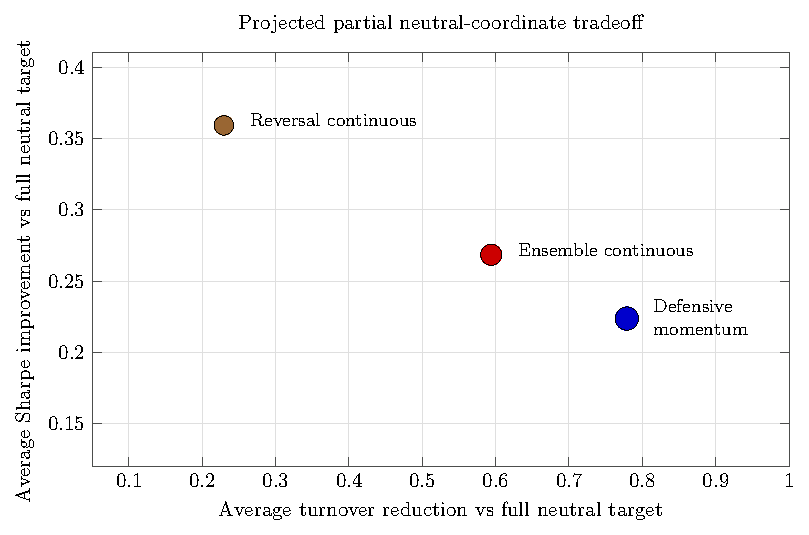
\includegraphics[width=0.84\linewidth]{figures/neutral_coordinate_tradeoff_scatter.pdf}
\caption{Projected partial neutral-coordinate candidates compared with the full neutral target. The horizontal axis reports average turnover reduction, and the vertical axis reports average Sharpe difference. Marker size is proportional to average maximum-drawdown improvement.}
\label{fig:tradeoff}
\end{figure}


The Sharpe and drawdown columns are reported as implementation diagnostics.  The primary empirical
objects are exposure leakage, turnover, and the stability of the projected partial path after optimisation
and rebalancing.  The positive Sharpe differences in Table~\ref{tab:aggregate} indicate that the
turnover-saving variants do not mechanically sacrifice realised performance in these panels, while the
main construction result is the numerical enforcement of the monitored exposure constraints.

Per-universe rows are reported in Appendix~\ref{app:additional-diagnostics}, Table~\ref{tab:per-universe}.  The appendix table records the heterogeneity of turnover reduction across panels.


\FloatBarrier

The maximum exposure error among fixed neutral-coordinate candidates is $4.97\times10^{-15}$.  For comparison,
ordinary alpha has maximum exposure $14.312$ and residualised alpha has maximum exposure $2.785$ in
the same final table.  This provides the most direct empirical distinction between capital-space neutrality
and signal residualisation in the reported tests.

\subsection{Beta coefficients and neutral-coordinate conditioning}

Table~\ref{tab:beta-diagnostics} reports the partial-rebalance coefficient summaries for the three fixed
projected-partial candidates.  The coefficients are not simply a refusal to trade: the defensive candidate
has a binding cap by design, while the continuous candidates retain a substantial fraction of interior
choices.  Additional rank and conditioning checks for the neutral-coordinate basis are reported in Appendix~\ref{app:additional-diagnostics}.

\begin{table}[!htbp]
\centering
\small
\begin{tabular}{lrrrrrr}
\toprule
Strategy & Mean $\beta$ & Median $\beta$ & $\Pr(\beta=0)$ & $\Pr(\beta=1)$ & $\Pr(0<\beta<1)$ & Turnover \\
\midrule
Defensive momentum & 0.175 & 0.250 & 0.038 & 0.000 & 0.962 & 0.196 \\
Ensemble continuous & 0.315 & 0.120 & 0.097 & 0.183 & 0.720 & 0.362 \\
Reversal continuous & 0.465 & 0.230 & 0.095 & 0.379 & 0.526 & 0.682 \\
\bottomrule
\end{tabular}
\caption{Projected partial rebalancing coefficient summaries, averaged across the six universes in the fixed validation protocol.}
\label{tab:beta-diagnostics}
\end{table}


\subsection{Exposure specification and stress sensitivity}
\label{sec:exposure-specification}

The main validation uses $F_t=[1,\sigma,\sigma^2,\sigma^3]$.  The cubic volatility specification is used
because it gives a compact test of neutrality against both linear and nonlinear characteristic exposure
without introducing a large multi-factor risk model.  An order-sweep check confirms that
exact neutrality is not tied to the cubic exposure specification.  The construction remains neutral when
the exposure matrix is varied from $[1,\sigma]$ through $[1,\ldots,\sigma^4]$, with rank failures equal
to zero in the reported sweep.  The cubic specification is therefore used as the fixed validation choice
rather than as a mathematically privileged exposure order.  A stress test perturbs the exposure
model and compares the realised leakage with the finite-sample misspecification bound.



Detailed stress-test summaries are reported in Appendix~\ref{app:additional-diagnostics},
Table~\ref{tab:exposure-stress}.  The maximum bound ratio remains below one and the minimum
linearity $R^2$ is $0.970$, supporting the finite-sample misspecification bound in
Proposition~\ref{prop:combined-leakage-bound} without adding another main-text table.


\FloatBarrier

\subsection{Bootstrap uncertainty}


Appendix~\ref{app:additional-diagnostics}, Table~\ref{tab:bootstrap}, reports stationary-bootstrap uncertainty.  Turnover reductions are stable across all six universes for the defensive and ensemble candidates; Sharpe and drawdown comparisons are favourable but less uniform.  These results are consistent with the implementation-oriented scope of the study.


\FloatBarrier

\subsection{Transaction-cost sensitivity}



Figure~\ref{fig:cost} reports sensitivity to realised transaction-cost assumptions. The comparison is
relative to the full neutral target. As costs rise, the projected partial portfolios benefit from lower
turnover.

\begin{figure}[!htbp]
\centering
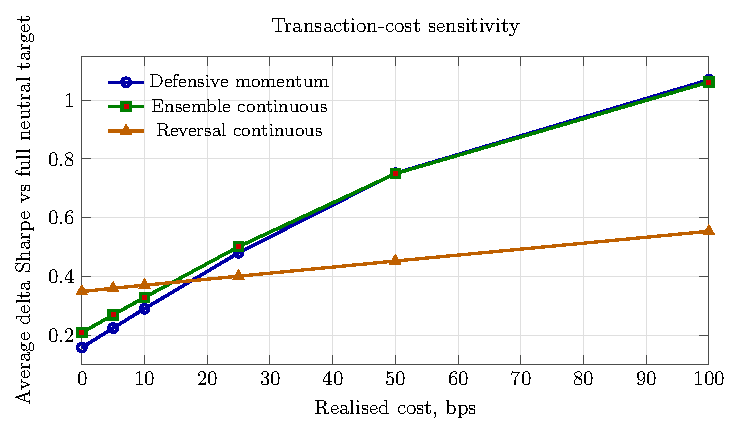
\includegraphics[width=0.84\linewidth]{figures/cost_sensitivity_delta_sharpe.pdf}
\caption{Transaction-cost sensitivity of the three fixed projected partial neutral-coordinate variants.  The vertical
axis reports average delta Sharpe versus the full neutral-coordinate target at the indicated
realised-cost assumption. The figure reports a relative turnover-control diagnostic under simple
realised-cost assumptions.}
\label{fig:cost}
\end{figure}

\FloatBarrier

Early, middle, and late subperiod checks are directionally consistent with the aggregate interpretation.
Turnover reductions persist across subperiods for the projected partial neutral-coordinate candidates, while Sharpe
and drawdown improvements are favourable but less uniform.  This supports the paper's main
implementation claim without turning the subperiod split into a second model-selection exercise.

\FloatBarrier
\section{Research data audit and implementation diagnostics}

The empirical panels are processed validation panels used to evaluate the portfolio-construction layer.
The neutrality checks are computed directly from the implemented weights and the recorded exposure
matrices at each rebalance.  Country and Style have local OHLCV proxy coverage with volume and
spread-proxy fields, while GlobalCountries has partial OHLCV proxy coverage for the available overlap.
The US large-cap sample, Sector, and USBonds are cleaned level-only panels in the current data files.
The US large-cap sample contains 48 series and is used as a fixed large-cap research sample.

\begin{table}[!htbp]
\centering
\scriptsize
\begin{tabular}{lllp{2.35in}}
\toprule
Universe & Source type & Volume/spread proxy & Diagnostics used \\
\midrule
Country & local proxy OHLCV panel & yes & construction + cost-accounting check \\
GlobalCountries & local proxy OHLCV panel & partial & construction + partial cost-accounting check \\
US large-cap sample & cleaned level panel & no & construction and neutrality checks \\
Sector & cleaned level panel & no & construction and neutrality checks \\
Style & local proxy OHLCV panel & yes & construction + cost-accounting check \\
USBonds & cleaned level panel & no & construction and neutrality checks \\
\bottomrule
\end{tabular}
\caption{Research data-audit scope.  The table records which checks are available in the replication files for the processed research panels.}
\label{tab:data-scope}
\end{table}

The monitor records neutrality, selected beta, turnover, ex-ante risk, condition number, drawdown,
monitoring flags, weights, and trade lists at every rebalance.  The maximum monitored neutrality error is
$4.94\times10^{-15}$; after scalar volatility targeting it is $6.00\times10^{-15}$, in line with
Proposition~\ref{prop:scalar-overlays}.  These values support the scalar-overlay invariance result without
requiring a separate monitor table.

Proxy cost-accounting checks were computed only for panels where local OHLCV proxy fields are
available, including partial coverage for GlobalCountries. These checks validate turnover and
cost-accounting implementation; the detailed rows are included with the replication supplement rather
than used as a main manuscript result.

\FloatBarrier
\section{Discussion}

The empirical results support the finite-sample construction claim.  Neutral-coordinate portfolios have
exposure leakage at numerical precision, while ordinary and residualised-alpha portfolios retain material
exposure after optimisation and rebalancing.  This distinction is the main practical point of the paper:
residualising a signal and enforcing neutrality on the traded capital vector are different operations.

The projected partial portfolios illustrate the role of the projection step.  When the exposure matrix
changes through time, the previous holding is not generally neutral under the new exposure matrix.
Projecting the old holding into the current neutral subspace creates a neutral starting point for the new
rebalance.  The subsequent interpolation controls turnover while remaining inside the monitored neutral
subspace.

The performance statistics provide implementation context.  In the reported panels, projected partial
neutral-coordinate portfolios reduce turnover relative to the full neutral target while preserving
capital-level neutrality.  The same construction layer can be combined with richer alpha models,
commercial or internal risk models, and stricter liquidity and capacity controls.  Its role is to enforce the
selected exposure policy on the implemented portfolio after optimisation, scaling, and rebalancing.

\section{Scope and extensions}

The construction guarantees are finite-sample and exposure-relative.  Given the monitored exposure
matrix $F_t$, the neutral-coordinate portfolio lies in $\ker F_t^\top$, and the projected partial
rebalancing path remains in the same current-date neutral subspace.  The method therefore enforces the
selected exposure policy on the implemented capital vector.

The empirical study uses fixed research panels, simple signal definitions, trailing covariance estimates,
and a parsimonious volatility-exposure specification.  These choices keep the validation focused on the
construction layer.  A production implementation can use a richer alpha model, a commercial or internal
risk model, broader exposure definitions, liquidity constraints, and more detailed transaction-cost models
without changing the neutral-coordinate construction.

The exposure matrix remains an investment-policy choice.  The method enforces neutrality with respect
to the columns included in $F_t$.  Additional style, sector, country, beta, liquidity, or nonlinear
characteristic exposures can be incorporated by adding columns to the monitored exposure matrix,
subject to the available degrees of freedom in the universe.

\section{Conclusion}

This paper developed a finite-sample construction method for imposing factor neutrality on implemented
portfolio weights.  The key distinction is between residualising an alpha signal and constraining the
capital vector that is actually traded.  Signal residualisation can help interpret a forecast, but neutrality
for an active sleeve is a property of the implemented weights after optimisation, scaling, and
rebalancing.

At each rebalance, the exposure matrix $F_t$ defines the monitored neutral capital subspace
$\ker F_t^\top$.  Writing the portfolio as $u_t=Q_t\theta_t$ restricts the optimiser to that subspace and
gives the same capital vector as a Markowitz problem with equality constraints.  The same representation
yields finite-sample exposure-leakage bounds when the construction and monitoring exposure matrices
differ.

The rebalancing rule projects the previous holding into the current neutral subspace before trading
toward the new neutral target.  A partial trade is then taken along the line segment between the
projected holding and the full neutral target.  Since both endpoints are neutral under the current
exposure matrix, the entire interpolation path remains neutral.

In the reported walk-forward tests, neutral-coordinate portfolios have exposure leakage at numerical
precision.  The projected partial variants reduce turnover relative to the full neutral target while
preserving capital-level neutrality.  The construction provides a transparent way to implement and audit
factor-neutral mandates at the level of traded capital weights.

\section*{Conflicts of Interest}

The author declares no conflicts of interest.

\section*{Data and code availability}

The empirical tables and figures are generated from research code implementing neutral-coordinate
construction, projected partial rebalancing, and exposure-monitoring checks.  Code sufficient to reproduce
the reported tables and figures from the processed research panels will be provided as supplementary
material or through an anonymised repository during review.  Source data subject to vendor or licence
restrictions are not redistributed.

\FloatBarrier
\appendix
\section{Additional technical and audit checks}
\label{app:additional-diagnostics}

This appendix records the projection ablation, fixed implementation protocol, per-universe rows,
exposure-stress checks, stationary-bootstrap uncertainty, and rank-conditioning checks.  Additional
replication files include transaction-cost accounting details, subperiod summaries, exposure-order
sweeps, monitor logs, and proxy cost-accounting rows.

\subsection{Projection ablation: why partial rebalancing must start inside the current neutral subspace}
\label{app:projection-ablation}

The following ablation isolates the role of the projection step.  Suppose the manager starts from the previous implemented portfolio $u_{t-1}$ and partially rebalances directly toward the current full neutral target $u_t^*\in\N_t$, without first projecting $u_{t-1}$ into the current neutral subspace.  The resulting unprojected path is
\begin{equation}
    \widetilde u_t(\beta)=(1-\beta)u_{t-1}+\beta u_t^*,\qquad 0\leq \beta\leq 1.
\end{equation}
Since $F_t^\top u_t^*=0$, its current-date exposure is
\begin{equation}
    F_t^\top \widetilde u_t(\beta)=(1-\beta)F_t^\top u_{t-1}.
\end{equation}
Thus the unprojected path is current-date neutral only if $\beta=1$ or the old holding already lies in the new neutral subspace $\N_t$.  In walk-forward use, $F_t$ changes with the exposure estimates, so yesterday's neutral portfolio need not be neutral under today's exposure matrix.  The projected rule fixes this problem: with
\begin{equation}
    u_{t-1\to t}=\Pi_{\N_t}u_{t-1},\qquad
    u_t(\beta)=(1-\beta)u_{t-1\to t}+\beta u_t^*,
\end{equation}
one has $F_t^\top u_t(\beta)=0$ for every $\beta\in[0,1]$.  The projection step is therefore required for exact capital-level neutrality under changing exposure definitions.

\begin{table}[!htbp]
\centering
\small
\begin{tabular}{lp{4.25in}}
\toprule
Component & Fixed validation specification \\
\midrule
Rebalance frequency & Approximately monthly, implemented as 21-trading-day walk-forward rebalances. \\
Lookback window & 252 trailing trading days, using only information available before the holding interval. \\
Exposure matrix & $F_t=[1,\sigma_t,\sigma_t^2,\sigma_t^3]$ in the fixed validation; $\sigma_{i,t}$ is the 252-day trailing volatility computed before the holding interval. \\
Risk estimate & Trailing covariance matrix with ridge regularisation in the optimisation step. \\
Signals & 63-day momentum, 252-day momentum skipping 21 days, 21-day reversal, EWMA trend, volatility-scaled momentum, and equal-weight ensemble signals. \\
Fixed candidates & Defensive momentum, ensemble continuous, and reversal continuous neutral-coordinate. \\
Partial-rebalance rule & One-dimensional utility maximisation over $\beta\in[0,1]$. \\
Turnover penalty & Common fixed ex-ante coefficient $7500$; it is held fixed across universes and candidates and was not chosen by universe-level performance tuning.  The defensive candidate additionally caps $\beta$ at $0.25$. \\
Transaction-cost sensitivity & Reported at 0, 5, 10, 25, 50, and 100 basis points. \\
Universe-specific retuning & None in the fixed validation. \\
\bottomrule
\end{tabular}
\caption{Fixed implementation protocol.  The table records the information set, candidate definitions, and common validation choices used in the final comparison.}
\label{tab:implementation-protocol}
\end{table}

\begin{table}[!htbp]
\centering
\scriptsize
\begin{tabular}{lrrrrrr}
\toprule
Universe & Hard S & Mom S & Mom TO red. & Ens. S & Ens. TO red. & Rev. S \\
\midrule
Country & -0.107 & 0.048 & 0.746 & 0.075 & 0.462 & 0.105 \\
GlobalCountries & -0.490 & -0.059 & 0.745 & 0.047 & 0.546 & 0.499 \\
US large-cap & -0.181 & -0.006 & 0.745 & 0.193 & 0.635 & 0.282 \\
Sector & -0.237 & 0.117 & 0.804 & 0.159 & 0.661 & 0.321 \\
Style & -0.067 & -0.055 & 0.812 & 0.046 & 0.606 & -0.060 \\
USBonds & 0.094 & 0.307 & 0.821 & 0.101 & 0.654 & 0.020 \\
\bottomrule
\end{tabular}
\caption{Per-universe fixed neutral-coordinate comparison.  ``S'' denotes Sharpe and ``TO red.'' denotes turnover reduction versus the full neutral-coordinate target.}
\label{tab:per-universe}
\end{table}

\begin{table}[!htbp]
\centering
\small
\begin{tabular}{lrrrr}
\toprule
Universe & Max bound ratio & Median bound ratio & Min linearity $R^2$ & Stress pass rate \\
\midrule
Country & 0.664 & 0.093 & 0.989 & 1.000 \\
GlobalCountries & 0.579 & 0.081 & 0.983 & 1.000 \\
US large-cap & 0.460 & 0.047 & 0.970 & 1.000 \\
Sector & 0.837 & 0.222 & 0.994 & 1.000 \\
Style & 0.763 & 0.115 & 0.989 & 1.000 \\
USBonds & 0.796 & 0.304 & 0.986 & 1.000 \\
\bottomrule
\end{tabular}
\caption{Exposure-stress linearity and leakage-bound checks.  The table summarises perturbed-exposure tests and supports the combined numerical and misspecification bound in Proposition~\ref{prop:combined-leakage-bound}.}
\label{tab:exposure-stress}
\end{table}

\begin{table}[!htbp]
\centering
\scriptsize
\begin{tabular}{llrrrr}
\toprule
Strategy & Metric & Avg delta & Win rate & CI excludes 0 & N \\
\midrule
Defensive momentum neutral-coordinate & Sharpe & 0.224 & 0.869 & 2 & 6 \\
Defensive momentum neutral-coordinate & Turnover & -0.689 & 1.000 & 6 & 6 \\
Defensive momentum neutral-coordinate & Max drawdown & 0.173 & 0.997 & 6 & 6 \\
Ensemble continuous neutral-coordinate & Sharpe & 0.268 & 0.861 & 3 & 6 \\
Ensemble continuous neutral-coordinate & Turnover & -0.524 & 1.000 & 6 & 6 \\
Ensemble continuous neutral-coordinate & Max drawdown & 0.139 & 0.927 & 1 & 6 \\
Reversal continuous neutral-coordinate & Sharpe & 0.359 & 0.737 & 2 & 6 \\
Reversal continuous neutral-coordinate & Turnover & -0.203 & 0.938 & 4 & 6 \\
Reversal continuous neutral-coordinate & Max drawdown & 0.124 & 0.812 & 1 & 6 \\
\bottomrule
\end{tabular}
\caption{Stationary-bootstrap comparison against the full neutral-coordinate target.  CI counts are the number of universes, out of six, where the 95 percent bootstrap interval excludes zero.  Win rates are computed in the favourable direction: higher Sharpe, lower turnover, or improved maximum drawdown.}
\label{tab:bootstrap}
\end{table}

\begin{table}[!htbp]
\centering
\small
\begin{tabular}{lrrrrr}
\toprule
Universe & Median rank $F_t$ & Min $d_t$ & Median $d_t$ & Median condition & Max leakage \\
\midrule
Country & 4 & 6 & 6 & 2.106 & $7.12\times10^{-16}$ \\
GlobalCountries & 4 & 12 & 12 & 3.563 & $1.54\times10^{-15}$ \\
US large-cap & 4 & 44 & 44 & 9.584 & $2.65\times10^{-15}$ \\
Sector & 4 & 7 & 7 & 1.028 & $4.81\times10^{-16}$ \\
Style & 4 & 6 & 6 & 2.032 & $6.48\times10^{-16}$ \\
USBonds & 4 & 9 & 9 & 6.019 & $9.07\times10^{-16}$ \\
\bottomrule
\end{tabular}
\caption{Rank and conditioning checks for the main candidate monitor.  Here $d_t=\dim\ker F_t^\top$ and the condition statistic is the monitored neutral-risk condition number for the neutral-coordinate risk problem.}
\label{tab:rank-conditioning}
\end{table}

\FloatBarrier
\clearpage

\begin{thebibliography}{99}

\bibitem[Boyd et~al.(2017)]{Boyd2017}
Boyd, S., Busseti, E., Diamond, S., Kahn, R.N., Koh, K., Nystrup, P. and Speth, J. (2017)
`Multi-period trading via convex optimization', \emph{Foundations and Trends in Optimization}, Vol. 3, No. 1, pp.1--76.

\bibitem[Clarke et~al.(2002)]{ClarkeDeSilvaThorley2002}
Clarke, R., de Silva, H. and Thorley, S. (2002)
`Portfolio constraints and the fundamental law of active management', \emph{Financial Analysts Journal}, Vol. 58, No. 5, pp.48--66.

\bibitem[DeMiguel et~al.(2009)]{DeMiguel2009}
DeMiguel, V., Garlappi, L. and Uppal, R. (2009)
`Optimal versus naive diversification: how inefficient is the 1/N portfolio strategy?', \emph{Review of Financial Studies}, Vol. 22, No. 5, pp.1915--1953.

\bibitem[Grinold and Kahn(2000)]{GrinoldKahn2000}
Grinold, R.C. and Kahn, R.N. (2000) \emph{Active Portfolio Management}, 2nd ed., McGraw-Hill, New York.

\bibitem[Jagannathan and Ma(2003)]{JagannathanMa2003}
Jagannathan, R. and Ma, T. (2003)
`Risk reduction in large portfolios: why imposing the wrong constraints helps', \emph{Journal of Finance}, Vol. 58, No. 4, pp.1651--1683.

\bibitem[Kolm et~al.(2014)]{Kolm2014}
Kolm, P.N., Tutuncu, R. and Fabozzi, F.J. (2014)
`60 years of portfolio optimization: practical challenges and current trends', \emph{European Journal of Operational Research}, Vol. 234, No. 2, pp.356--371.

\bibitem[Ledoit and Wolf(2004)]{LedoitWolf2004}
Ledoit, O. and Wolf, M. (2004)
`Honey, I shrunk the sample covariance matrix', \emph{Journal of Portfolio Management}, Vol. 30, No. 4, pp.110--119.

\bibitem[Lobo et~al.(2007)]{Lobo2007}
Lobo, M.S., Fazel, M. and Boyd, S. (2007)
`Portfolio optimization with linear and fixed transaction costs', \emph{Annals of Operations Research}, Vol. 152, No. 1, pp.341--365.

\bibitem[Markowitz(1952)]{Markowitz1952}
Markowitz, H. (1952)
`Portfolio selection', \emph{Journal of Finance}, Vol. 7, No. 1, pp.77--91.

\bibitem[Michaud(1989)]{Michaud1989}
Michaud, R.O. (1989)
`The Markowitz optimization enigma: is optimized optimal?', \emph{Financial Analysts Journal}, Vol. 45, No. 1, pp.31--42.

\bibitem[Politis and Romano(1994)]{PolitisRomano1994}
Politis, D.N. and Romano, J.P. (1994)
`The stationary bootstrap', \emph{Journal of the American Statistical Association}, Vol. 89, No. 428, pp.1303--1313.

\end{thebibliography}

\end{document}
